\chapter{Observation Interface}
\label{ch:ui}

% Sources: thesis-pack/07-observation-ui/ui-README.md (data flow, WebSocket
% protocol, animation pipeline, HTTP endpoints, notify-reset handshake, layout),
% adr/0005 (Postgres as single source of truth), adr/0017 Decision 2 (headless
% client instead of self-acknowledgement). Written as built. Identifiers: table
% and message names only, no code file names.

The agents of Chapter~\ref{ch:agentic} run as ten separate programs, and they
meet only in the database (Chapter~\ref{ch:data}). A running simulation is
therefore hard to follow from the outside. In this chapter we describe the
observation interface, a small web application that shows a live agentic run
on a map of Hamburg. It is supporting material. It helped us build and debug
the agents, and it gives a reader a way to look at a single decision. It
played no part in scoring.

% =====================================================================
\section{Purpose}
\label{sec:ui:goals}

The interface has two jobs. The first is to show a run as it happens: where
each vehicle is, which step each agent is working on, and which messages are
moving between them. The second is to make each reasoning step inspectable.
When an agent does something unexpected, we can open the exact prompt it
received and the exact answer the model gave. This is how we found most of the
faults in the agents while we built them.

The interface makes no decisions. Each agent is the only writer of
its own state row, and the interface never changes it. The interface writes to
the database in three places only. It records the world's acknowledgements
when a vehicle finishes a drive (Section~\ref{sec:ui:ack}). It enqueues the
scenario's events into the agents' mailboxes. And it clears the run tables when
the operator resets the simulation. Because all state lives in PostgreSQL, a
restart of the interface loses nothing. The backend reads the states again,
and a browser that reconnects receives fresh snapshots.

The interface serves only the agentic system. The workflow baseline has no
live view. It runs from its own command-line tool
(Section~\ref{sec:wf:cli}), and its vehicles are moved by its execution model
(Section~\ref{sec:wf:world}), so it needs no map to close a drive.

% =====================================================================
\section{Backend}
\label{sec:ui:backend}

The backend is a Python web service built on FastAPI. It sits between the
database and the browser and has four parts. Figure~\ref{fig:ui:dataflow}
shows how data moves between them.

% Data flow between the agents, the database, the UI backend and the browser.
% Source: thesis-pack/07-observation-ui/ui-README.md ("How data moves",
% "Animation Pipeline", "HTTP Endpoints"). Input from inc/ui.tex,
% Section "Backend".
\begin{figure}[htbp]
\centering
\begin{tikzpicture}[
  wide/.style={draw, rounded corners=2pt, text width=12.4cm,
    minimum height=0.9cm, align=center, font=\footnotesize},
  tab/.style={draw, rounded corners=2pt, fill=orange!8, text width=2.75cm,
    minimum height=0.7cm, align=center, font=\footnotesize},
  be/.style={draw, rounded corners=2pt, fill=gray!10, text width=2.75cm,
    minimum height=0.9cm, align=center, font=\footnotesize},
  box/.style={draw, dashed, rounded corners=3pt, inner sep=5pt},
  wr/.style={-{Stealth[length=1.8mm]}, thick, gray!70!black},
  lbl/.style={font=\scriptsize, align=left, text=gray!30!black},
  title/.style={font=\scriptsize\bfseries, anchor=south west},
]
  % --- agents, top -------------------------------------------------------
  \node[wide, fill=blue!6] (ag) at (5.1,0) {%
    \textbf{Ten agent programs}\\
    {\scriptsize each saves its own state, reads its mail and its world reports}};

  % --- database tables ----------------------------------------------------
  \node[tab] (st) at (0,-2.4)   {\texttt{states}};
  \node[tab] (ms) at (3.4,-2.4) {\texttt{messages}};
  \node[tab] (we) at (6.8,-2.4) {\texttt{world\_events}};
  \node[tab] (ts) at (10.2,-2.4){\texttt{tick\_sidecars}};
  \node[box, fit=(st)(ts)] (db) {};
  \node[title] at (db.north west) {PostgreSQL};

  % --- UI backend ------------------------------------------------------------
  \node[be] (wa) at (0,-4.9)   {ten watchers\\{\scriptsize diff, send changes}};
  \node[be] (di) at (3.4,-4.9) {scenario\\dispatcher};
  \node[be] (ac) at (6.8,-4.9) {acknowledgement\\endpoint};
  \node[be] (ti) at (10.2,-4.9){tick record\\endpoint};
  \node[box, fit=(wa)(ti)] (bk) {};
  \node[title] at (bk.north west) {UI backend};

  % --- browser, bottom --------------------------------------------------------
  \node[wide, fill=green!6] (br) at (5.1,-7.4) {%
    \textbf{Browser}\\
    {\scriptsize map with vehicle animations, agent panel, tick drawer}};

  % --- column 1: state out ------------------------------------------------------
  \draw[wr] (ag.south -| st) -- node[lbl, right] {save,\\then NOTIFY} (st.north);
  \draw[wr] (st.south) -- node[lbl, right] {wake,\\read} (wa.north);
  \draw[wr] (wa.south) -- node[lbl, right] {WebSocket:\\snapshots, changes,\\routed commands} (br.north -| wa);

  % --- column 2: scenario in -------------------------------------------------------
  \draw[wr] (di.north) -- node[lbl, right] {scenario\\events} (ms.south);
  \draw[wr] (ms.north) -- node[lbl, right] {NOTIFY,\\wake} (ag.south -| ms);

  % --- column 3: acknowledgements back ---------------------------------------------
  \draw[wr] (br.north -| ac) -- node[lbl, right] {\texttt{task\_complete},\\real position} (ac.south);
  \draw[wr] (ac.north) -- node[lbl, right] {append} (we.south);
  \draw[wr] (we.north) -- node[lbl, right] {NOTIFY,\\close leg} (ag.south -| we);

  % --- column 4: prompt records ------------------------------------------------------
  \draw[wr] (ag.south -| ts) -- node[lbl, right] {prompt and\\answer} (ts.north);
  \draw[wr] (ts.south) -- (ti.north);
  \draw[wr] (ti.south) -- node[lbl, right] {on demand,\\over HTTP} (br.north -| ti);
\end{tikzpicture}
\caption[How data moves through the observation interface]{How data moves through the observation interface. Each column is one
path. State goes out from the agents to the browser. Scenario events go into
the agents' mailboxes. Acknowledgements come back from the browser's animations
and become the agents' world reports. Prompt records are fetched only when a
tick is opened. Every path passes through the database, and the interface never
writes an agent's state.}
\label{fig:ui:dataflow}
\end{figure}


\paragraph{Watchers.} There is one watcher for each of the ten agents. A
watcher reads its agent's row in the \texttt{states} table and compares it
with the last version it has seen. It then sends only the keys that changed.
The watcher does not poll in a loop. It waits for the notification that the
agent sends on its state channel after each save, with the same five-second
fallback that the agents use (Section~\ref{sec:data:notify}). Until an agent
has saved its first state, the watcher checks every half second.

\paragraph{One WebSocket.} All updates reach the browser over one WebSocket
connection. When a browser connects, it first receives the current snapshot of
every agent. After that it receives only the changes. Each message names the
agent it belongs to. The four agents that move a vehicle also produce
commands, for example ``drive the bus to this address''. Before the backend
sends such a command, it adds a road route from OpenRouteService, the target
coordinates and the expected duration. When the routing service fails, the
route falls back to a straight line, and the map draws that line in red so
the fallback is visible.

\paragraph{Scenario dispatcher.} When a run starts, the dispatcher loads the
chosen scenario file. It uses the same loader as the workflow baseline, so both
systems read every scenario in the same way (Chapter~\ref{ch:validity}). The
dispatcher then waits until each event's simulated time and writes the event
into the recipient's mailbox in the \texttt{messages} table. The wait follows
the same time scale that the agents read, so the dispatcher, the agents' clocks
and the map animation stay in step.

\paragraph{Simulation control.} The operator can start, stop and reset a run.
A start creates a new run identifier and passes it to all ten agent programs,
together with the number of residents given in the scenario. Every row the
agents write to the event log then carries this run. A start is refused when
the database cannot be reached or when a run is already active. A reset stops
all ten agents and empties the run tables: the states, the mailboxes, the
world reports, the prompt records and the timers. The event log is never
touched, because it is append-only (Section~\ref{sec:data:eventlog}).

% =====================================================================
\section{Frontend}
\label{sec:ui:frontend}

The frontend is a React application written in TypeScript. The map uses
Leaflet with OpenStreetMap tiles, and one central store keeps a separate part
for each agent. Figure~\ref{fig:ui:main} shows the screen during a run.

\begin{figure}[htbp]
\centering
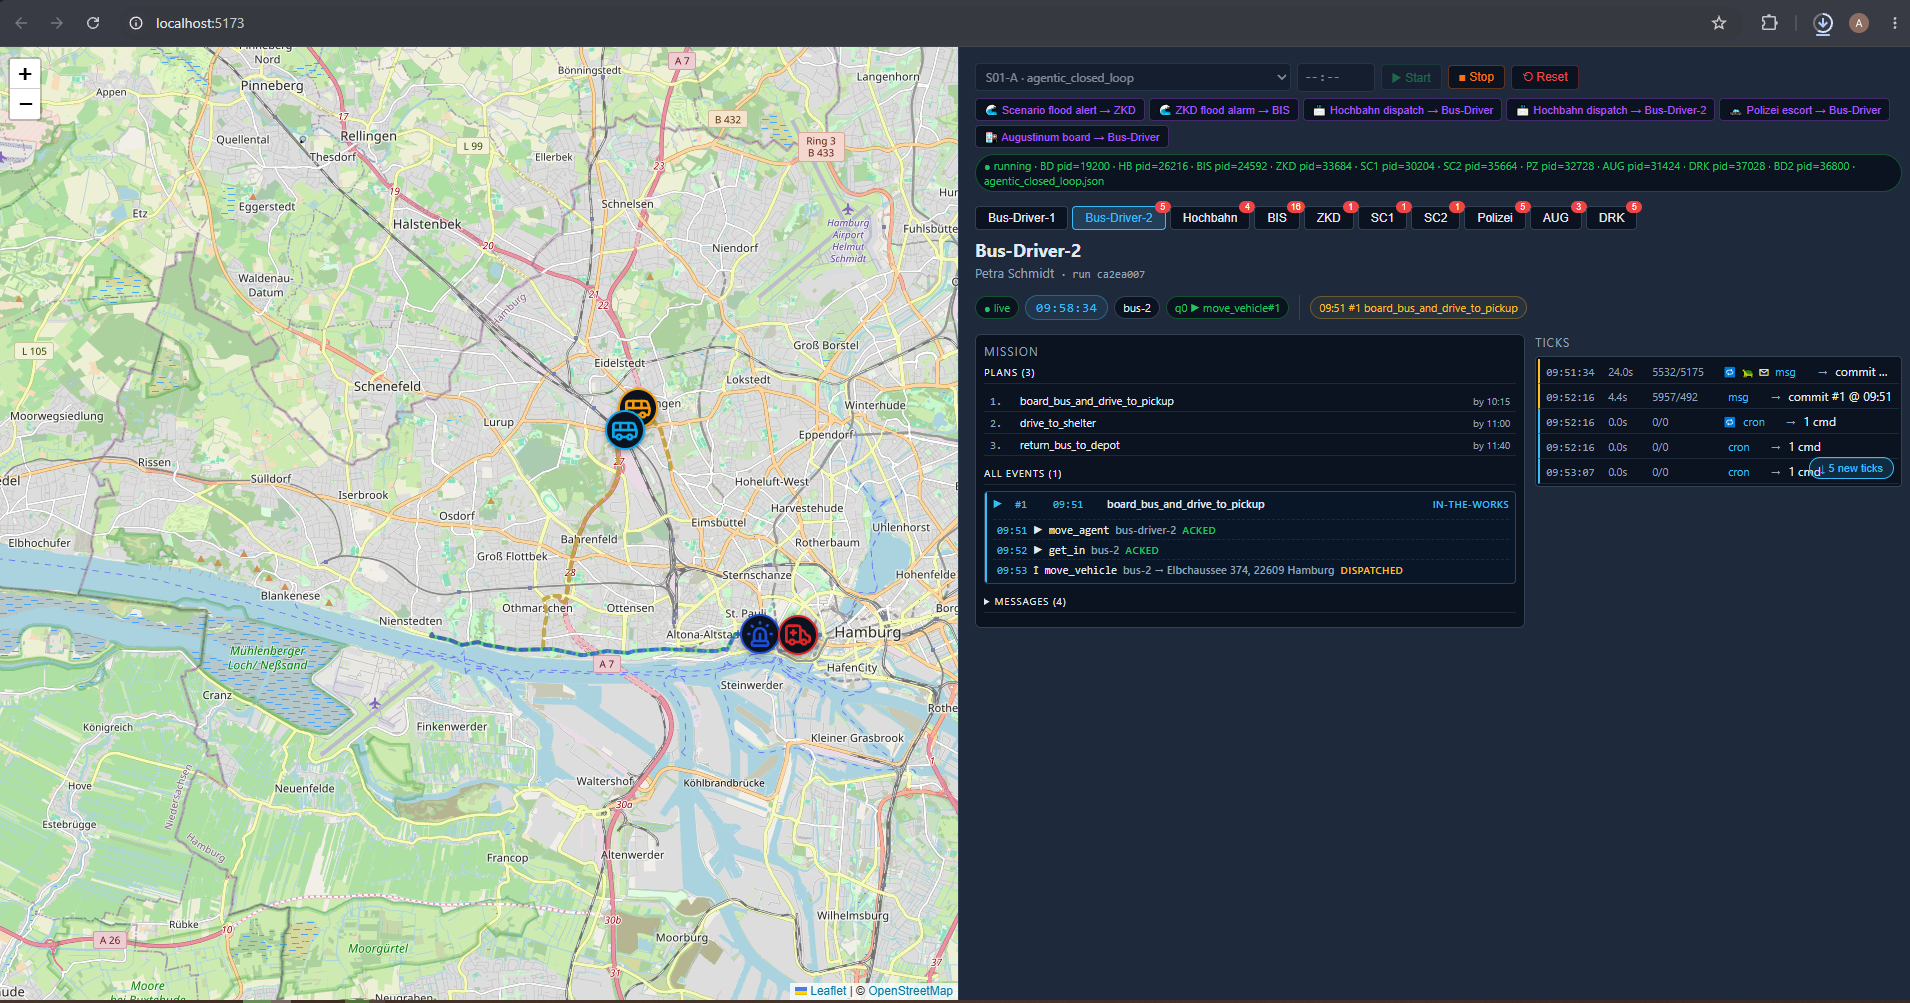
\includegraphics[width=\textwidth]{pics/ui-main.png}
\caption{The observation interface during a run of the undisrupted scenario.
Left: the map of Hamburg with the two buses, the police escort car and the
ambulance, each on its own route. Right, from the top: scenario selection and
run controls, the process identifiers of the ten agents, one tab per agent,
and the panel of the selected agent. Here this is Bus-Driver-2, with its three
planned steps and their deadlines, the actions of its current step with their
status, and its list of reasoning ticks.}
\label{fig:ui:main}
\end{figure}

\paragraph{The map.} The left half of the screen is the map. Each vehicle has
its own marker and colour, and its current route is drawn as a line. When the
backend sends a command, the frontend puts it in a queue for that vehicle. An animation then moves the marker along the route. The animation reads the
same time scale as the agents, so the map and the agents' clocks agree on how
long a drive takes.

\paragraph{The agent panel.} The right half has one tab for each agent.  The panel
of a vehicle driver shows the current simulated time, the vehicle it uses, its
remaining plan with a deadline for each step, and the actions of its current
step. Each action carries a status, such as dispatched or acknowledged. The coordinating agents move no vehicle, so their
panels show their state without one. Next to the plan, a list shows every tick
of the agent: when it started, what woke it, how long the model took, how many
tokens it used and what it committed.

\paragraph{The tick drawer.} A click on a tick opens a drawer with its full
record (Figure~\ref{fig:ui:tick}). The drawer shows what woke the agent, the
system prompt and the user prompt that the model received, the raw answer of
the model, and the plan the runtime read from that answer. This record is not
sent over the WebSocket. The browser fetches it from the \texttt{tick\_sidecars}
table only when a tick is opened.

\begin{figure}[htbp]
\centering
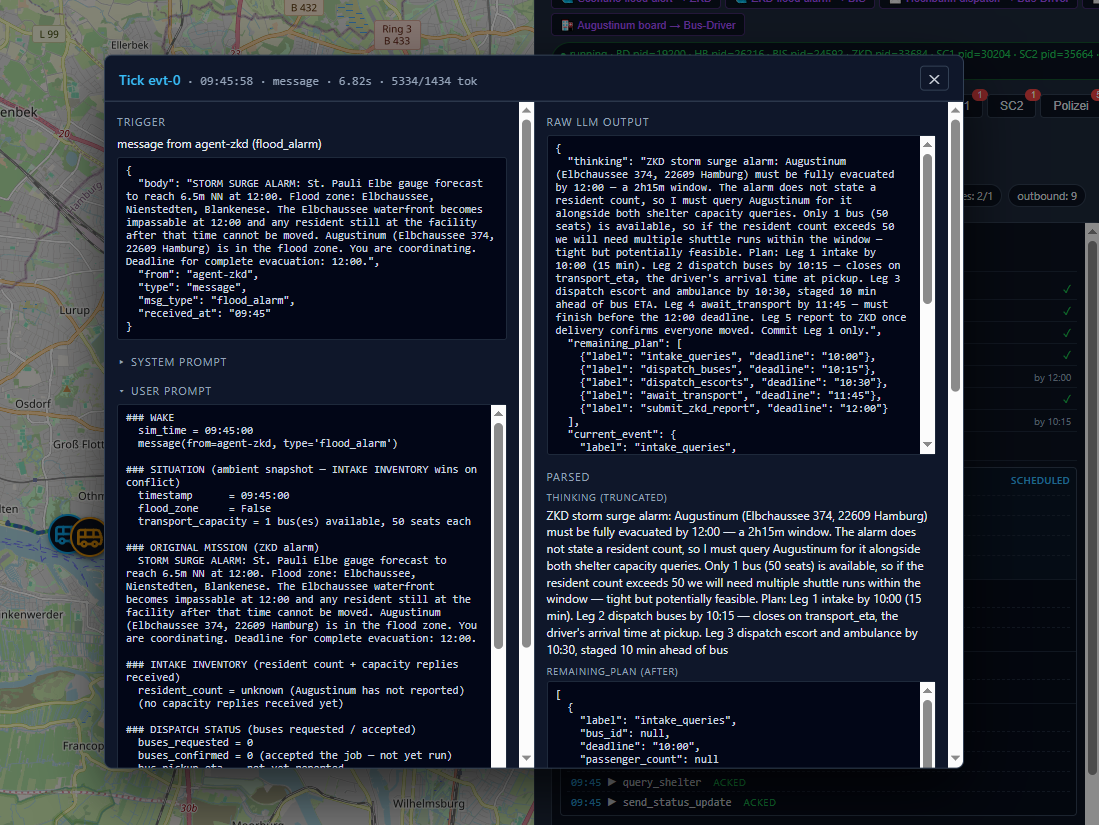
\includegraphics[width=0.9\textwidth]{pics/ui-tick-drawer.png}
\caption{The tick drawer for one reasoning tick of BIS, woken by the storm
surge alarm from ZKD. Left: the trigger message and the prompts the model
received. Right: the raw model output and the parts the runtime parsed from it,
here the model's reasoning and its new remaining plan. The header gives the
simulated time, the latency (6.82\,s) and the input and output tokens.}
\label{fig:ui:tick}
\end{figure}

For research, the drawer is the most useful part of the interface. A reader
who doubts a decision can open the tick behind it and see what the agent knew
and what the model wrote. The prompt records are cleared with the next reset,
so this view serves a live or just-finished run. The event log keeps its own
rows for every decision.

For testing, the controls also offer a row of buttons that send one message by
hand, for example a flood alert to ZKD or a dispatch order from Hochbahn to a
bus driver. A message sent this way goes into the mailbox like any other
message, and it is accepted only while a run is active.

% =====================================================================
\section{The Acknowledgement Channel}
\label{sec:ui:ack}

There is one place where the interface does more than watch. A drive is closed only when
the world confirms that it is finished (Section~\ref{sec:ag:runtime}). During a
live run, the browser's animation plays the role of the world.

When a vehicle's animation reaches the end of its route, the frontend sends a
\texttt{task\_complete} message back to the backend. The message carries the
command's number, the vehicle and the vehicle's final position. The backend
decides from the vehicle which agent owns it: the first bus and the car belong
to Bus-Driver-1, the second bus to Bus-Driver-2, the patrol car to Polizei and
the ambulance to DRK. It then appends the acknowledgement to that agent's
\texttt{world\_events}. The agent wakes, closes the step and takes its real
position from the report. If an agent changes its plan while a vehicle is
still moving, the animation stops, and the frontend sends a
\texttt{vehicle\_halted} message with the position where the vehicle stopped.
This message only updates the location. It does not mark any action as done.

Because of this loop, the interface matters for the evaluation even though
it scores nothing. A run with no acknowledgement source has no bus that ever
arrives.

% =====================================================================
\section{Runs Without a Browser}
\label{sec:ui:headless}

The evaluation runs its cells one after another, and no browser is open
during them. For these runs a headless world client replaces the browser
(Section~\ref{sec:eval:harness}). It follows the commands the backend emits
and sends the same kind of acknowledgement at the end of each drive.

We could have let the engine acknowledge its own commands instead. We decided
against this. A self-acknowledging engine would remove the handshake with the
world that an agent has to complete, and the evaluation would then score the
architecture on a property it does not have.

Two acknowledgement sources must never run at the same time, because every
drive would then be counted twice. Before each agentic cell, the harness
therefore sends a reset notice to the interface backend. The backend forwards
it to every open browser tab. A tab that receives it clears its stored state
and reloads, so it does not keep showing the old run over empty tables. The
backend also replies with the number of connected tabs. If any tab is
connected, the cell does not start. If no interface backend is running, the
notice fails quietly and the cell starts as normal.

% =====================================================================
\section{Summary}
\label{sec:ui:summary}

The observation interface shows a live agentic run on a map of Hamburg and
lets a reader open the full record of any reasoning tick. A backend watches
each agent's state through database notifications and sends only the changes
to the browser over one WebSocket. The interface does not decide anything and
never writes an agent's state. Its one active role is to acknowledge finished
drives, and in the evaluation a headless client takes over this role with the
same messages. Since an evaluation cell refuses to start while a browser tab is open, the
scored runs were produced without the interface in the loop.
